We start by showing the result of the computation using the full matrices.
We limited ourselves to grayscale images for the beginning and for computing the entire matrices, we can only process small images.
The image below contains 135 000 pixels, so each matrix need around 145 GB.

\begin{figure}[H]
  \centering
  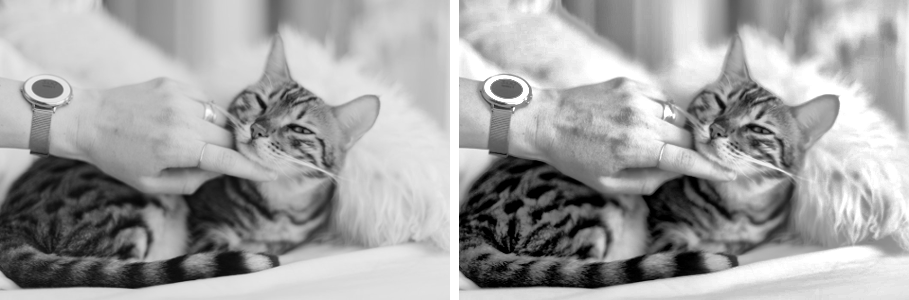
\includegraphics[width=0.95\textwidth]{img/cat.png}
  \caption{Left: input image. Right: sharpened image.}
\end{figure}

The cat's fur on the left-hand side and the hand appear to be more detailed.
We observe that the already sharp parts on the cat's head stay nice but some over-sharpening artifacts appeared in the background.
We obtained this filter by defining \(f(\Lapl) = -3\Lapl\) in the output image \(z = (I - f(\Lapl))y\).

This corresponds to the adaptive sharpening operator defined in \cite{siam_slides_2016} as \((I + \beta \Lapl)\) with \(\beta > 0\).
This approach remains a simple application of a scalar and it doesn't require any eigenvalue computation.
A more complete approach is called multiscale decomposition \cite{talebi_nonlocal_2014} and consists of applying a polynomial function to the Laplacian \(\Lapl\).
We apply different coefficients to different eigenvalues of \(\Lapl\) because each eigenpair captures different features of the image.
